\documentclass[10pt]{article}
\usepackage{graphicx}
\usepackage[backend=biber,style=numeric,sorting=ynt]{biblatex}

\addbibresource{references.bib}

\title{Prism Spectrometer} % Write the name of the experiment here
\author{Rahmanyaz Annyyev, Hikmat Gulaliyev} % Members of the lab group
 
\date{02 March 2024} % Date of the report

% The best place to start is overleaf.com. It is a web based LaTeX editor that allows you to write your report in a web browser. It also has a built in compiler that will typeset your document into a PDF. In order to start using overleaf, you need to create an account, create project and upload the report template to overleaf. Once you do that, you are good to go. You can also download the LaTeX editor of your choice and use that to write your report.


\begin{document}
\maketitle

\begin{abstract}
In this experiment, we utilize a prism spectrometer---an optical device that separates light into its constituent frequencies---to measure the refractive index of a prism. A collimator with a slit is used to produce a parallel beam of light emitted by a mercury lamp, which is then passed through the prism. The light is then refracted and dispersed into its constituent frequencies. The angle of deviation of the light is measured and used to calculate the refractive index of the prism using a special relation. A graph of the index of refraction versus wavelength is also plotted. The results are compared to the theoretical values and the limitations of the experiment are discussed.
\end{abstract}

\section{Introduction}
The visible spectrum is the portion of electromagnetic radiation that is visible to the human eye. It is composed of light with wavelengths between 380 and 740 nm. Each wavelength, or frequency of light is perceived as a different color by the human eye. 



A prism spectrometer is an optical device that separates the visible spectrum into its constituent frequencies. It is composed of a collimator with an adjustable slit, a prism resting on a rotating table, and a telescope with an adjustable crosshair. 

The collimator is used to produce a parallel beam of light emitted by a mercury lamp. The light is then passed through the prism, which refracts and disperses the light into its constituent frequencies. The telescope is used to observe the light and measure the angle of deviation of the light. The angle of deviation is then used to calculate the refractive index of the prism using a special relation. The refractive index of a prism is a measure of how much the light is bent when it passes through the prism. The refractive index of a prism is a function of the wavelength of the light. The refractive index of a prism is given by the following relation:




Each frequency of light is perceived as a different color by the human eye. The prism spectrometer is used to measure the refractive index of a prism and to plot a graph of the refractive index versus wavelength. The refractive index of a prism is a measure of how much the light is bent when it passes through the prism. The refractive index of a prism is a function of the wavelength of the light. The refractive index of a prism is given by the following relation:


In the introduction you should give a brief overview of the experiment. You should start with a brief description of the theoretical background behind the experiment. You should also mention the methods used in the experiment. You are expected to cite your sources\cite{Bravyi_2020} midtext.\footnote{More information on how to do this can be found in the references section.}

%You can use the '\footnote' command to add a footnote to your document.

You can insert an inline equation using the \$ sign. As in $E=mc^2$. To display an equation in the middle of the page use the following:

\begin{equation}
    \int \frac{1}{x} dx = \ln|x| + C
\end{equation}

\section{Data \& Results}

\begin{table}[ht]
    \centering
    \begin{tabular}{|c|c|c|c|}
        \hline
        Something & Something & Something & Something \\
        \hline
        1234 & 1234 & 1234 & 1234 \\
        \hline
    \end{tabular}
    \caption{This is a caption for the table.}
    \label{tab:ex}
\end{table}

\begin{figure}[ht]
    \centering
    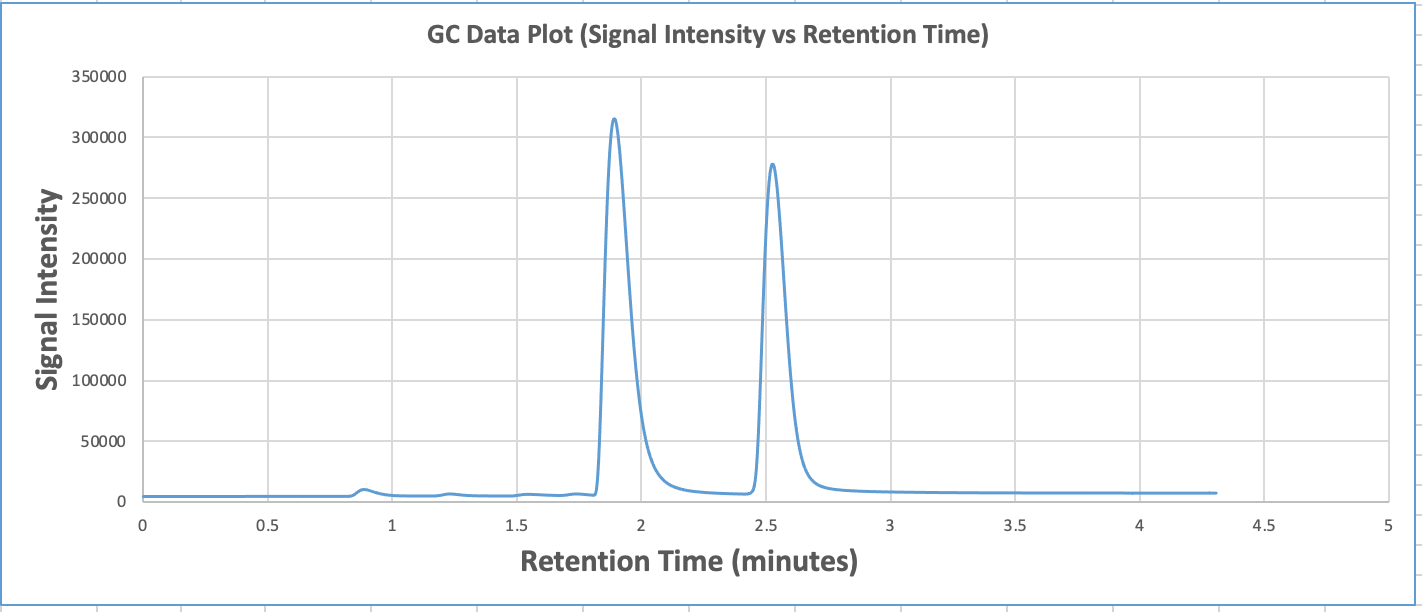
\includegraphics[width=0.72\textwidth]{example_figure.png}
    \caption{This is a caption for the figure.}
    \label{fig:ex}
\end{figure}

In this section, you are to present the data you obtain from the experiment,which is mostly going to be presented in the form of a table as in Table \ref{tab:ex} or in the form of a graph as in Figure \ref{fig:ex}. The manuals for the experiments have instructions on how to present the data, and in the case of any ambiguity you TA will provide you with the necessary information. You should also include any calculations you do in this section. A brief discussion of the results should also be included.

\section{Discussion \& Conclusion}

In this section, you are expected to discuss the limitations of the experiment and how these limitations may have affected the results. Meaning, you are to discuss the possible errors, the approximations you made in obtaining physical data, and the discrepancies you see between the results you obtain and the theoretical values or the values reported in the literature. You should also discuss the possible improvements that can be made to the experiment. 

\printbibliography

% You should put your references in the references.bib file. You can use an  online bibtex generator to generate the bibtex entry for your reference. You can cite your references in the text using the \cite{reference_title} command. The '\printbibliography' command will print the bibliography at the end of the document. 

\end{document}